\chapter{ATIVIDADES DESENVOLVIDAS}

Este capítulo descreve as atividades que foram realizadas no projeto desenvolvido durante o estágio. O estagiário realizou 352 horas de estágio, no período de 23 de maio a 02 de setembro de 2016.

\section{Ambientação e treinamento}
Durante as primeiras semanas do estágio, houve um período de ambientação sobre os projetos desenvolvidos na empresa, metodologias utilizadas e ferramentas. 

Durante a ambientação, o estagiário fez treinamento de Git\footnote{https://git-scm.com}, um sistema de controle de versão distribuído, e um sistema de gerenciamento de código fonte, com ênfase em velocidade. 

As atividades inicias foram focadas em atualizações e melhorias dos portais da empresa.

\section{Desenvolvimento front-end}
Simultaneamente aos trabalhos no projeto do software de planejamento estratégico, demandas de front-end surgiram, principalmente na criação de portais e manutenção dos existentes. A atuação como desenvolvedor front-end possibilitou a utilização das linguagens HTML5, CSS3, Javascript e o framework Bootstrap para a criação e manutenção de soluções online.

Um dos websites desenvolvidos foi o portal de apresentação do software. Foi desenvolvido utilizando as linguagens HTML5, CSS3, Javascript, Bootstrap e Hightcharts. O processo de desenvolvimento consistiu em levantamento de requisitos, formulação de conteúdo, prototipação, implementação e testes. O objetivo do portal é apresentar o software de uma forma clara e concisa, apresentando o projeto, as instituições participantes e estatísticas de pesquisas, em uma página de conversão única chamada ladingpage. Para a demonstração de dados coletados no desenvolvimento do projeto em forma de gráficos, foi necessário a utilização do framework Highcharts.

O Highcharts\footnote{http://www.highcharts.com} é um software de criação de web gráficos que produz gráficos animados utilizando JavaScript e HTML5 SVG. Ele funciona em todos os navegadores modernos e é exclusivamente com base em tecnologias de navegador nativo, isto é, não requer a instalação de plugins e extensões como Flash ou Java.


\section{Análise e especificação de requisitos}
Os requisitos do software eram coletados em reuniões com o cliente. Esses dados eram estudados e discutidos pela equipe e a especificação era realizada, através de documentações e protótipos.

Durante todas as etapas de desenvolvimento, os gestores do projeto, que também utilizarão o sistema no futuro, acompanhavam e homologavam as especificações e os protótipos desenvolvidos.

\section{Prototipação}

% TODO - a parte dos conceitos deveria ir para o capítulo anterior - aqui você descrever como foi a sua atividade***done!

Durante todo o desenvolvimento do software, os wireframes, mockups e protótipos foram criados para serem validados junto ao cliente e, ao mesmo tempo, sendo uma referência útil à equipe de programadores.

Após a análise e especificação, os protótipos ajudam a ter a primeira noção de como o sistema irá se parecer. Os protótipos serviram para os clientes validarem o que a equipe de especificação e design especificaram e, também, aos desenvolvedores, ajudando no momento da implementação. Os protótipos são uma aproximação de uma experiência que permite o usuário fazer uma simulação de como o produto em questão será.

Inicialmente, os protótipos foram baseados em wireframes e mockups, com o objetivo de demonstrar como os dados ficariam organizadas na interface.  

Um grande aprendizado durante a elaboração dos protótipos foi a de especificar as telas com dados que reaproximassem de dados reais. Isso permitiu ter uma abordagem mais concisa sobre os dados e, além disso, facilitava a homologação.

\subsection{Protótipo de baixa fidelidade}

O wireframe, como representa a Figura \ref{fig:wireframe} é uma representação de baixa fidelidade de uma interface. Foi reproduzido digitalmente.

\begin{figure}[H]
\centering
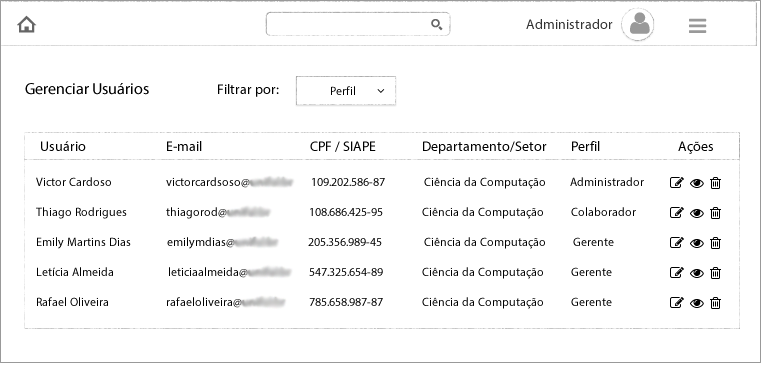
\includegraphics[width=1\textwidth]{images/wireframe.png}
\caption{Wireframe inicial}
\label{fig:wireframe}
\end{figure}

\subsection{Protótipo de alta fidelidade}
O mockup é uma representação estática do design próximo ao produto final. O design do software passou por várias modificações até encontrar, juntamente com o cliente, a melhor solução para a disposição dos dados na interface. A Figura \ref{fig:dashboard0} mostra a primeira versão do Painel de bordo do sistema, local onde os dados são apresentados em forma de tabelas e gráficos. Assim como a Figura \ref{fig:dashboard0_1} apresenta uma variação do mockup após sugestões do cliente. 

\begin{figure}[H]
\centering
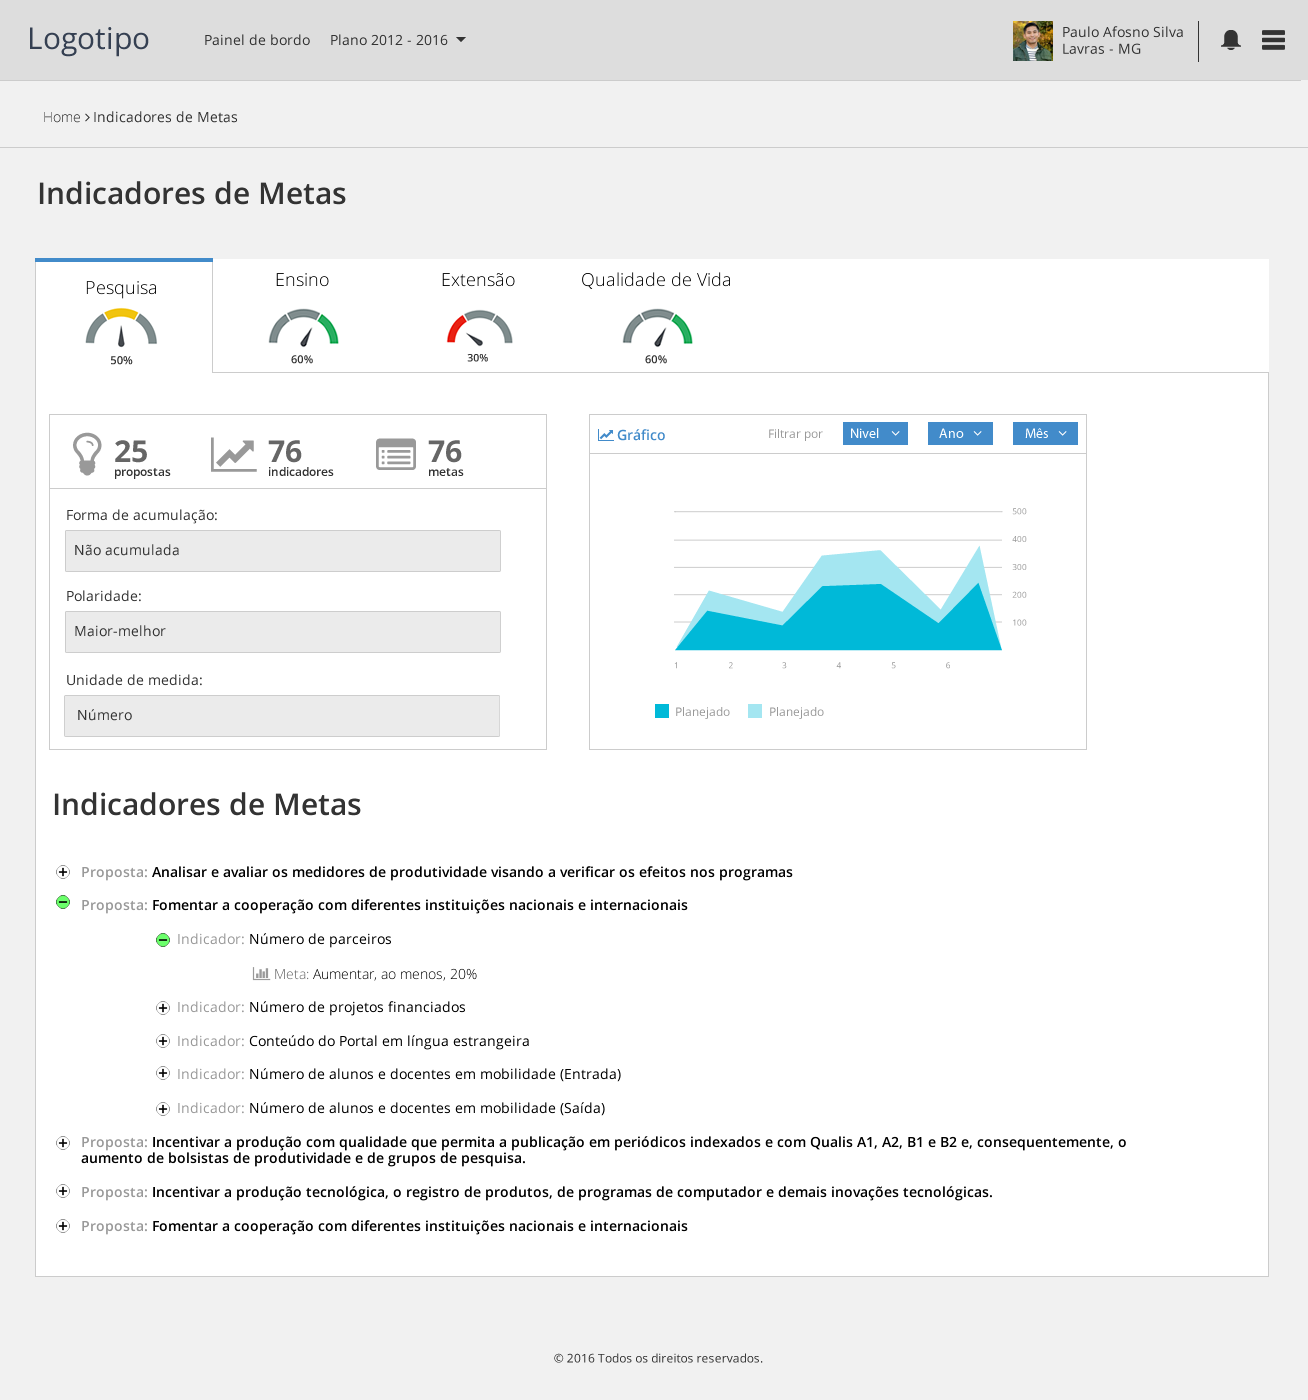
\includegraphics[width=1\textwidth]{images/dashboard0.png}
\caption{Mockup inicial}
\label{fig:dashboard0}
\end{figure}


\begin{figure}[H]
\centering
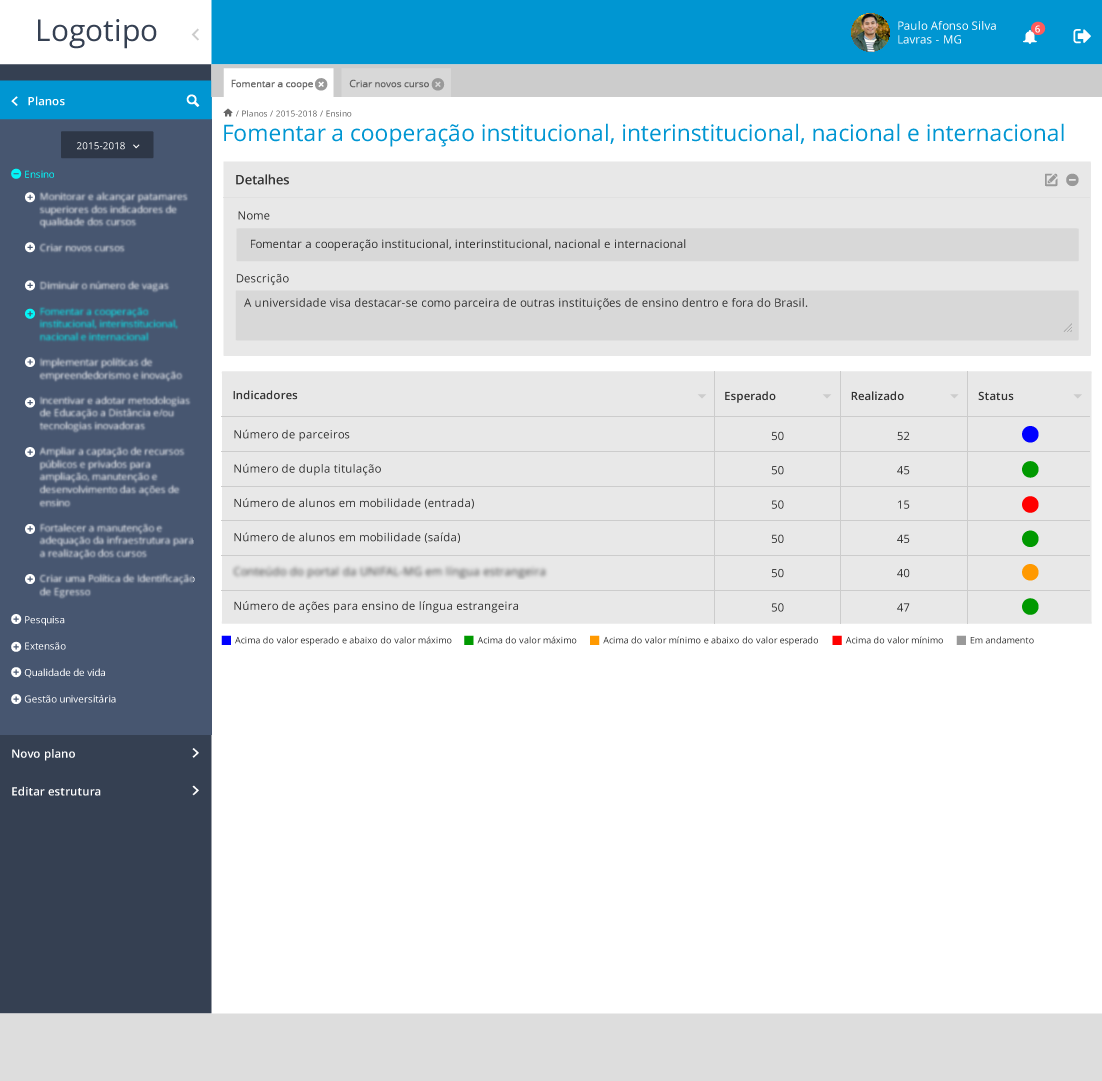
\includegraphics[width=1\textwidth]{images/dashboard0_1.png}
\caption{Segunda versão do mockup inicial}
\label{fig:dashboard0_1}
\end{figure}



Após uma série de ciclos, encontrou-se a melhor solução para o painel de bordo, utilizando um design limpo e com informações que seriam relevantes ao usuário.

%Informações removidas por serem confidenciais

% As Figuras \ref{fig:mockup11} e \ref{fig:mockup2} representam os mockups após estudos de viabilidade, modificações e reuniões com os clientes.

%\begin{figure}[H]
%\centering
%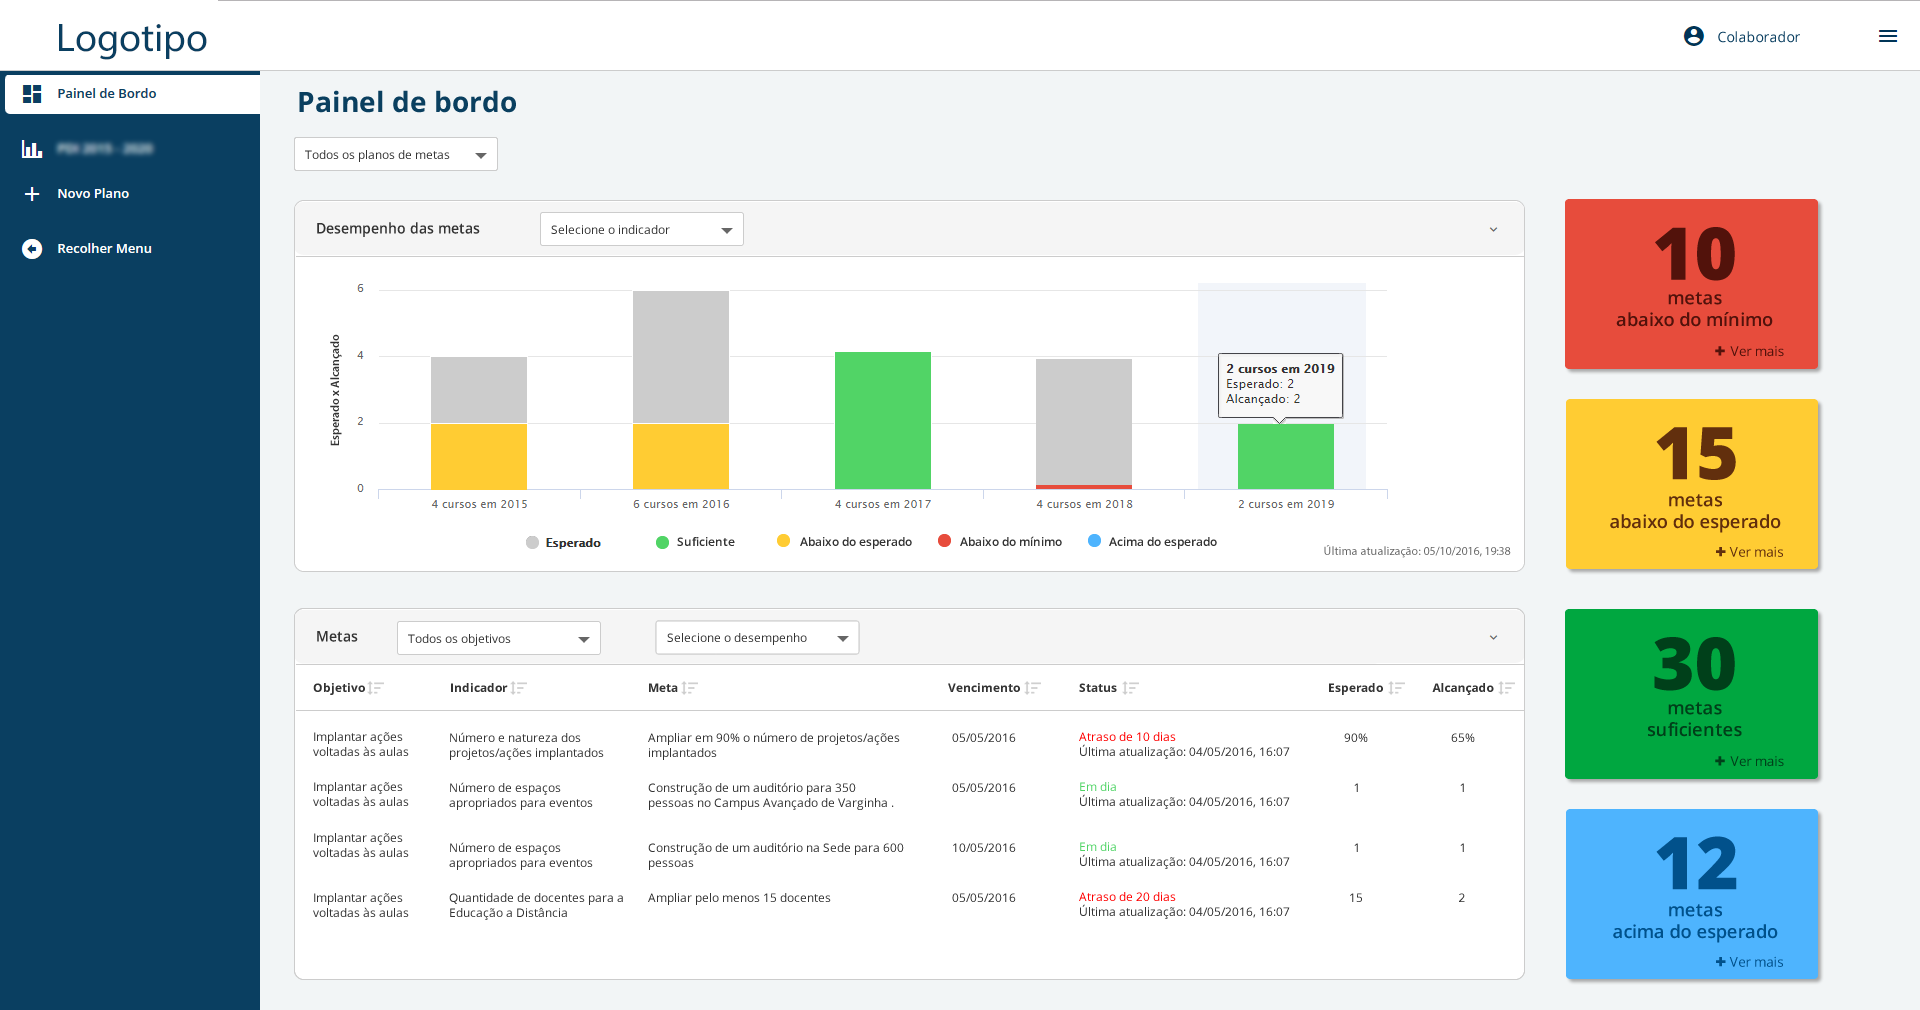
\includegraphics[width=1\textwidth]{images/mockup1.png}
%\caption{Mockup do Painel de bordo}
%\label{fig:mockup11}
%\end{figure}

%\begin{figure}[H]
%\centering
%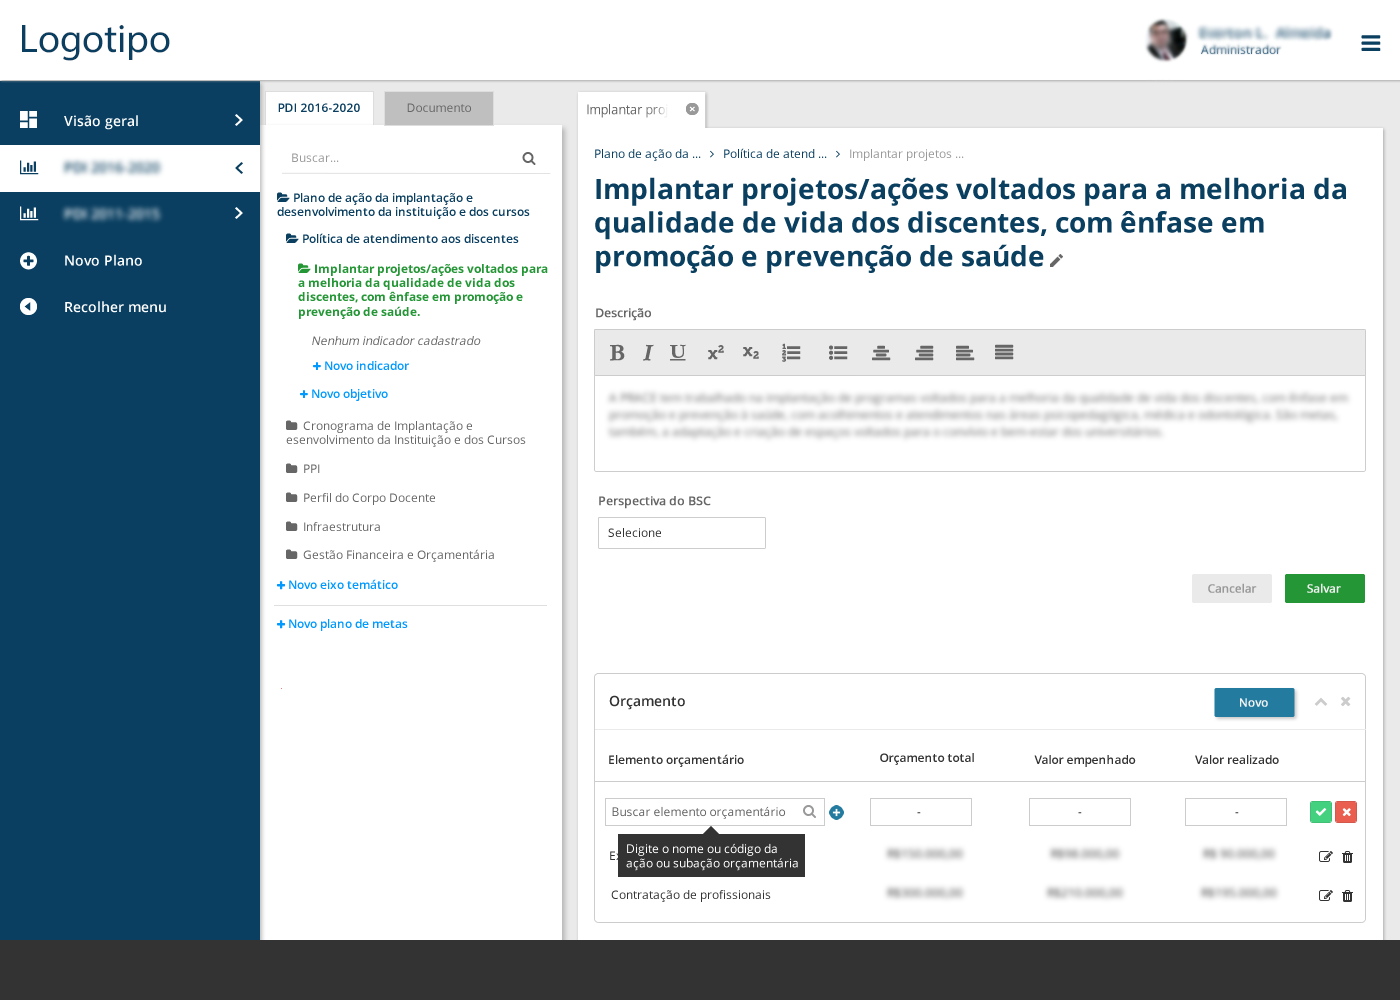
\includegraphics[width=1\textwidth]{images/mockup2.png}
%\caption{Mockup da estrutura}
%\label{fig:mockup2}
%\end{figure}

\subsection{Ferramentas utilizadas}
Os mockups e os wireframes foram desenvolvidos utilizando três softwares de manipulação de imagens diferentes, Adobe Photoshop versão CC, Adobe Fireworks versão CS6 e Adobe Illustrator versão CC. Para os protótipos dinâmicos, utilizou-se as ferramentas    MarvelApp e Axure versão RP.

\subsubsection{Adobe Illustrator}
O Adobe Illustrator\footnote{http://www.adobe.com/br/products/illustrator.html} é um editor de imagens vetoriais desenvolvido e comercializado pela Adobe Systems. Foi criado inicialmente para o Apple Macintosh em 1985 como complemento comercial de software de fontes da Adobe e da tecnologia PostScript desenvolvida pela empresa. Ele permite o desenvolvimento de imagens vetoriais.

\subsubsection{Adobe Photoshop}
O Adobe Photoshop\footnote{http://www.adobe.com/br/products/photoshop.html} é um software caracterizado como editor de imagens bidimensionais do tipo raster (possuindo ainda algumas capacidades de edição típicas dos editores, como Illustrator) desenvolvido pela Adobe Systems. É considerado o líder no mercado dos editores de imagem profissionais. Sua mais recente versão é o Adobe Photoshop CC, sua décima quarta edição 14.0

\subsubsection{Adobe Fireworks}
O Fireworks\footnote{http://www.adobe.com/br/products/fireworks.html} é um editor de imagens de bitmap e desenho vetorial desenvolvido pela Macromedia, posteriormente adquirido pela Adobe. Suas funcionalidades focam a publicação gráfica na Internet, por isso inclui suporte a GIF animado, PNG e imagens fatiadas, além de possuir ótima compressão de imagens. 

\subsubsection{MarvelApp}
 O MarvelApp\footnote{https://marvelapp.com} permite a criação de protótipos de alta fidelidade de maneira rápida, eficiente e portátil para testes realizados em smartphones. A partir de imagens e mockups, é possível transformá-los em protótipos para qualquer tipo de dispositivo, sem necessidade de codificação.

\subsubsection{Axure}
Soluções podem ser prototipadas e validadas pelas pessoas que melhor compreendem seus negócios, produtos e clientes. O Axure\footnote{https://www.axure.com} permite a criação de flowcharts, wireframes, mockups, personas e quadro de ideias. Além disso, permite uma maior interação juntamente com a entrada de dados pelo usuário.

\section{Desenvolvimento ágil}
Durante o desenvolvimento do projeto, foi utilizado o Trello\footnote{https://trello.com/} (Figura \ref{fig:trello}) como gerenciador de atividades da equipe. O Trello é um aplicativo de gerenciamento de projeto baseado na web, utilizando o paradigma Kanban para gerenciamento de projetos. Utilizando o Trello no projeto, as \textit{sprints} foram representadas pelos quadros (\textit{boards}), que contêm atividades. As atividades são representadas por cartões que são criados dentro dos quadros. Cada atividade é subdivida em tarefas, como um \textit{checklist}. No caso de especificação, as tarefas eram dividias em análise, especificação, design de interface e prototipação. Como vantagem, é possível representar o progresso da atividade, desta forma, a equipe tinha uma visão das atividades de todos, facilitando a comunicação.

As \textit{sprints} duravam de uma a três semanas, sendo que a duração mais comum era de duas semanas. No início de cada \textit{sprint}, a equipe se reunia para a reunião de \textit{planning}, onde as próximas atividades são apresentadas e a equipe divide as atividades em tarefas e estima quantas horas serão gastas para cada atividade. Durante o \textit{sprint}, havia reuniões diárias, chamadas de \textit{standup meeting} (reunião em pé, com o objetivo de serem rápidas), para cada membro da equipe falar o que foi desenvolvido, quais suas dificuldades e o que será desenvolvido posteriormente. E, ao final do \textit{sprint}, eram realizadas as reuniões de \textit{review} e \textit{retrospective}, para analisar se o objetivo do \textit{sprint} foi alcançado, e levantar os pontos fortes, pontos fracos e melhorias futuras. 

Observou-se que, ao utilizar essa metodologia durante o projeto, a comunicação entre os membros da equipe foi beneficiada e todos puderam ter uma noção do trabalho que estava sendo desenvolvido pelos outros. Outro fator importante a ser destacado foi a possibilidade de trabalho em conjunto das equipes de especificação, desenvolvimento e testes.

\begin{figure}[H]
\centering
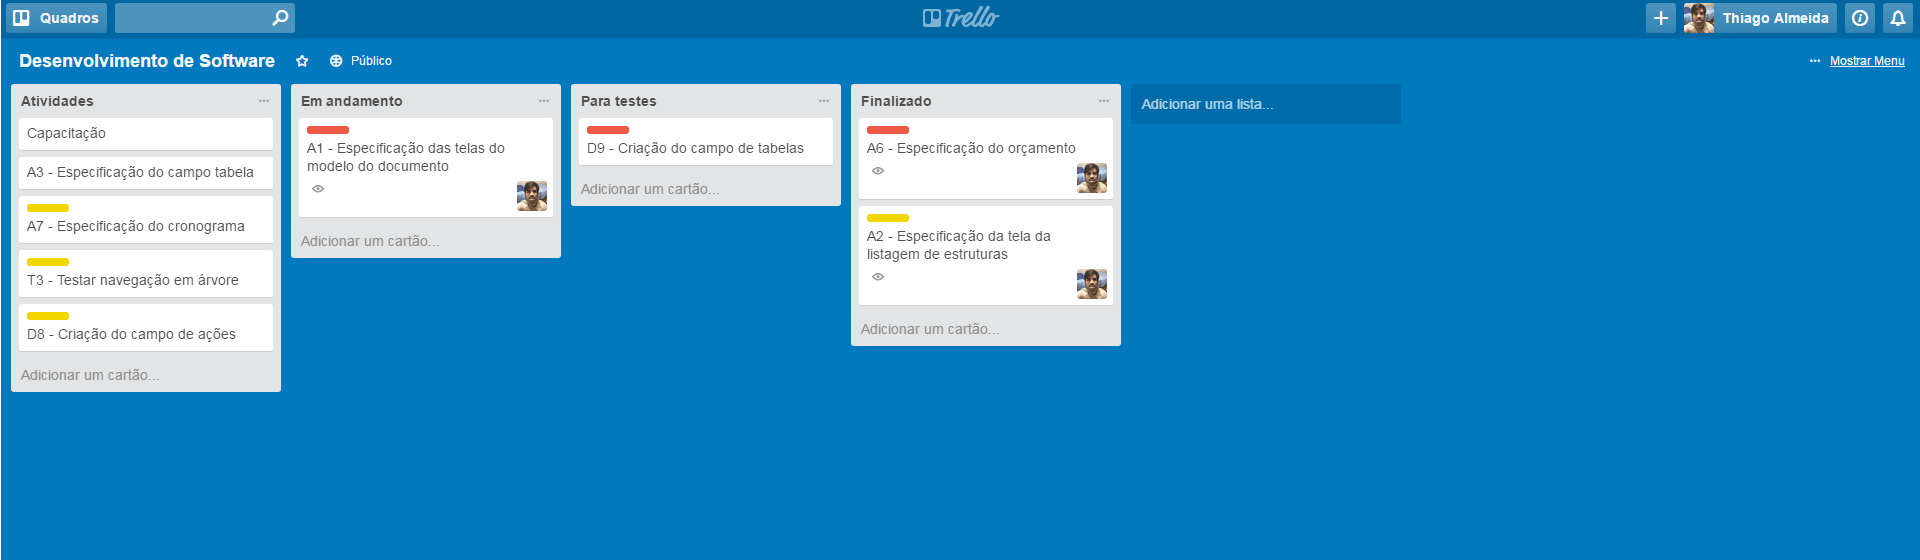
\includegraphics[width=1\textwidth]{images/trello.png}
\caption{Gerenciador de atividades - Trello }
\label{fig:trello}
\end{figure}


%\subsection{GitHub}
%GitHub é um serviço de Web Hosting Compartilhado para projetos que usam o controle de versionamento. Ele oferece funcionalidades como envio de código e correções, versionamento, issue tracker, entre outros.


%\section{personas}

%Foram consideradas personas do ForPDI  gestores, técnicos administrativos e professores de instituições federais de ensino superior. Os principais usuários do sistema serão os responsáveis pelo planejamento, elaboração, execução e acompanhamento do PDI da instituição de ensino. Haverá também a possibilidade da comunidade acessar alguns dados do sistema, acompanhando o andamento do PDI da instituição referente.

\section{Avaliação Heurística}

Foi realizada a avaliação heurística do software de planejamento estratégico na forma colaborativa, em duas sessões de 2 horas cada, com a participação de 5 especialistas em usabilidade. Sobre isso, Nielsen e Molich  \cite{Nielsen:1990:HEU:97243.97281} afirmam que os resultados de uma avaliação heurística serão muito melhores se houver várias pessoas conduzindo a avaliação, fazendo-a independentemente uns dos outros, e recomenda que a avaliação heurística seja feita com entre três e cinco avaliadores. A avaliação foi realizada em duas sessões, de aproximadamente 2 horas cada.
 

Foram consolidadas 5 tarefas a serem realizadas:

\begin{itemize}
\item login no sistema: nesta tarefa espera-se que o usuário realize o login no sistema (Obrigatório), recupere sua senha;
\item cadastro de domínio: nesta tarefa espera-se que o usuário cadastra o domínio;
\item cadastro de estrutura: nesta tarefa, espera-se que o usuário cadastre uma nova estrutura;
\item cadastro de plano estratégico: espera-se que o usuário cadastre um novo plano estratégico macro;
\item cadastro de plano de metas: nesta tarefa, espera-se que o usuário cadastre um novo plano de metas, cadastrando todo o fluxo de níveis,  a partir de um plano já cadastrado anteriormente. Será entregue um papel com as informações que devem ser inseridas em cada nível.
\end{itemize}

\subsection{Resultados}

Como resultado, obteve-se uma lista de problemas identificados, juntamente com as heurísticas afetadas, graus de severidade e, em muitos dos problemas, soluções propostas pelos avaliadores.

A partir da análise da avaliação heurística com especialistas da área, foram encontrados 118 problemas de usabilidade. Os dados referentes às violações categorizadas por severidade podem ser visualizados na Tabela ~\ref{tab:severidade}. A maioria dos problemas (83,78\%) foram classificados pelos avaliadores como problemas com severidade Simples (2). Em segundo lugar, com 41,3\%, foram classificados os problemas com severidade Sério (3). 

\begin{table}[H]
\centering
\caption{Severidades}
\label{tab:severidade}
\begin{tabular}{c|c|c}
      \hline
       \rowcolor[gray]{.9}
      \bf Severidade  & \bf Frequência & \bf Porcentagem  \\
      \hline
      \hline
0 (Não acredito que seja um problema) & 0          & 0\%         \\
1 (Cosmético)                        & 12         & 14,16\%     \\
2 (Simples)                          & 71         & 83,78\%     \\
3 (Sério)                           & 35         & 41,3\%      \\
4 (Catastrófico)                     & 0          & 0\%         \\

\hline
\hline
\bf TOTAL   & \bf 118        & \bf 100\%   \\
 \hline 
\end{tabular}
\end{table}



Entre os principais problemas elencados, destaca-se os relacionados a falta de \textit{feedback} e ajuda para o usuário. Não havia algum manual ou indicador de localização para que o usuário possa identificar o local onde está e o que deve fazer. Havia falta de \textit{feedbacks} quando o usuário realizava alguma ação no sistema, mesmo que a ação fosse realizada com sucesso. 

\begin{table}[H]
\centering
\caption{ Violações categorizadas por Heurísticas}
\label{tab:heuristicasAfetadas}
\begin{tabular}{c|c|c}
      \hline
      \rowcolor[gray]{.9}
 \bf Heurística   &  \bf Frequência & \bf Porcentagem  \\
      \hline
      \hline
H1. Visibilidade do status do sistema
& 10  & 7\%\\

H2. Correspondência entre o sistema e o mundo real 
& 15 & 10\% \\  

H3. Controle do usuário e liberdade                     
& 9  & 6\%     \\

H4. Consistência e padrões                          
& 29  & 19\%      \\

H5. Prevenção de erros                        
&15  & 10\%      \\

H6. Reconhecimento em vez de recordação                 
&3  &2\%      \\

H7. Flexibilidade e eficiência de utilização           
&5  &3\%      \\

H8. Estética e design minimalista                       
& 21  & 14\%      \\

H9. Ajude os usuários a reconhecer, diagnosticar e resolver erros                
& 15  &10\%      \\

H10. Ajuda e documentação                       
&15  &10\%      \\


\hline
\hline
\bf TOTAL   & \bf 137        & \bf 100\%   \\
 \hline 
\end{tabular}
\end{table}

A Heurística 4, consistência e padrões, obteve a maior frequência de problemas, com 29 ocorrências, representando 21\% das violações. A segunda maior violação foi a Heurística 8, estética e design minimalista, com 21 ocorrências, representando 15\% das violações. 

Em relação aos problemas que afetam a Heurística 4, consistência e padrões, o sistema apresentou padronizações diferentes para ações iguais, como larguras e alturas diferentes para elementos com as mesmas funções, padronização de campos, como data, sem máscara ou informar ao usuário, a forma correta e botões de salvar e cancelar aparecendo em diferentes lugares em contextos semelhantes.

A Heurística 8, estética e design minimalista, está relacionado a simplicidade da interface em relação à arquitetura da informação. Problemas como contraste de cores de ícones, campos pequenos ou muito grandes, textos muito grandes que tornam a tela com muitas informações, principalmente na árvores de níveis do software, foram encontrados.

E nas Heurísticas 9 e 10, ajude os usuários a reconhecer, diagnosticar e resolver erros, e ajuda e documentação, respectivamente,  observou-se a falta de ajuda no sistema sobre o que se tem que fazer. Por se tratar de formulários com grande quantidade de campos, e alguns específicos da área de planejamento institucional, observou-se a falta de informações sobre a funcionalidade do campo a ser preenchido. O sistema também não continha informações precisas sobre erros ao submeter uma informação no sistema.


\subsection{Melhorias implantadas}
Os problemas encontrados nos testes e nas avaliações heurísticas foram cadastrados no repositório do projeto, para serem corrigidos pela equipe. Um levantamento realizado três meses após a avaliação heurística mostrou que, dos 118 problemas de usabilidade encontrados, 87 foram resolvidos, totalizando 74\% de problemas corrigidos. O resultado esperado compreendeu as expectativas da equipe e dos gestores e seguiu o planejamento inicial do projeto. 

\subsubsection{Mensagens de alerta e erro}
Foram estabelecidas mensagens de erros, alertas e confirmações de quando há alguma mudança de contexto inesperada pelo usuário. Ao clicar no botão para deletar ou cancelar alguma ação, a mensagem de confirmação é importante para evitar que o usuário tenha clicado no botão erroneamente. Ao salvar algo, a mensagem de confirmação é mostrada ao usuário, como demonstrado na Figura \ref{fig:feedback1}. Quando o usuário comete algum erro de preenchimento nos formulários, além de mostrar uma mensagem dizendo que há erros, os erros são mostrados no específico lugar que ocorreu, como demonstrado na figura \ref{fig:erros}

\begin{figure}[H]
\centering
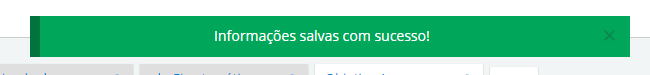
\includegraphics[width=1.1\textwidth]{images/feedback1.png}
\caption{Mensagem de confirmação}
\label{fig:feedback1}
\end{figure}

\begin{figure}[H]
\centering
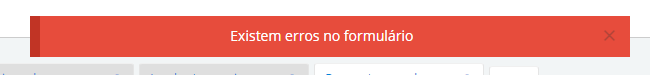
\includegraphics[width=1.1\textwidth]{images/erros.png}
\caption{Mensagem de erro}
\label{fig:erros}
\end{figure}

\subsubsection{Árvore de níveis}
A estrutura das ações, objetivos e indicadores de um planejamento estratégico é realizada por meio de níveis hierárquicos. Devido a esse fato, foi necessário desenvolver um cadastro que possibilitava o usuário visualizar qual o nível correto de cada informação. Para isso, o cadastro é realizado em forma de árvore de níveis. Após a avaliação heurística e discussão com os especialistas, a árvore foi modificada para atender melhor o usuário.

A Figura \ref{fig:arvore_geral} demonstra as três primeiras fases da evolução do design da árvore de níveis. Após estudos de viabilidade de implementação, e após a realização da avaliação heurística, a árvore foi passou por modificações, que pudessem atingir seus objetivos, com uma interface agradável ao usuário onde os dados pudessem ser organizados em forma hierárquica sem nenhuma complicação.

%Durante os ciclos de desenvolvimento, a árvore de níveis passou por modificações, como demonstrado na Figura \ref{fig:arvore_geral} que pudessem atingir seus objetivos, com uma interface agradável ao usuário. 


\begin{figure}[H]
\centering
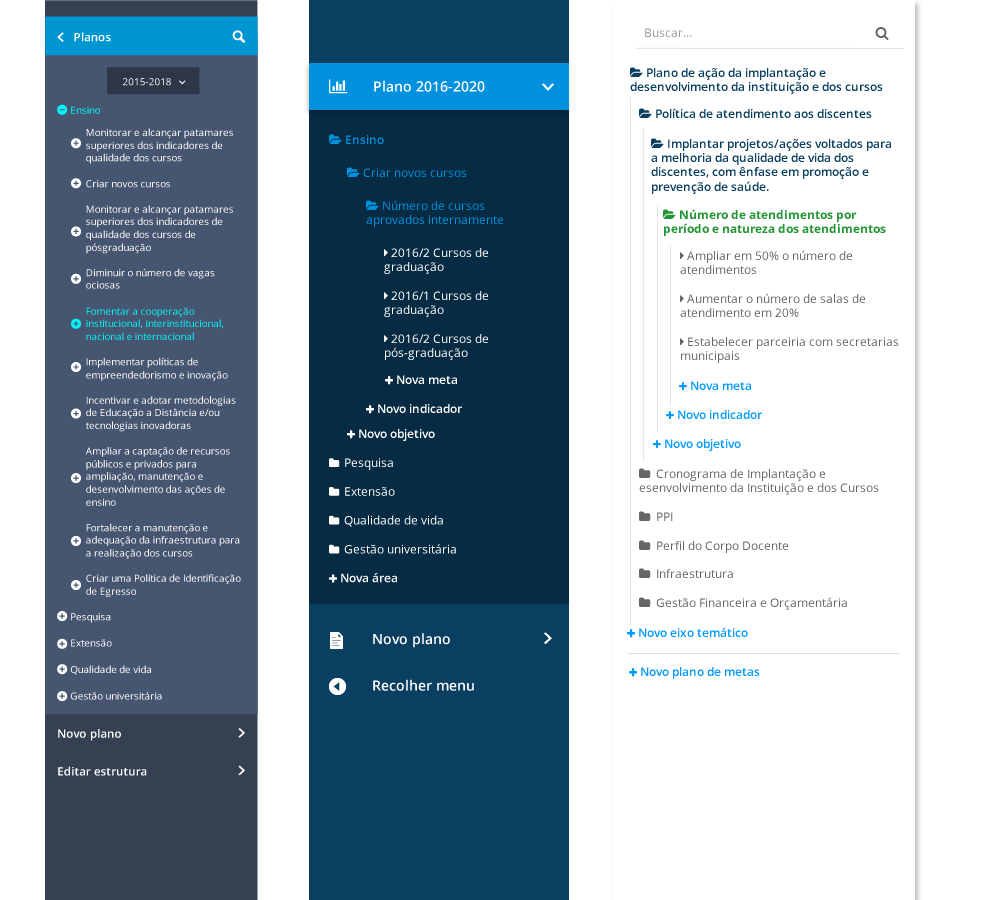
\includegraphics[width=1.1\textwidth]{images/arvore.png}
\caption{Evolução do design da árvore de níveis}
\label{fig:arvore_geral}
\end{figure}

\section{Design de interface}
Após algumas fases de análise e requisitos durante as \textit{sprints}, análises e estudos de softwares semelhantes, e avaliação heurística, o estilo de design do sistema foi estabelecido e homologado e, desde então, o software passou a ter seu estilo próprio de design, demonstrado na Figura \ref{fig:estilo}, como tamanho de fontes, tipografia, cores, formato de tabelas, gráficos e iconografia. O estilo de design permitiu o alinhamento entre as demandas de especificação e implementação. Os protótipos, que passaram a seguir o estilo de design, representavam fielmente como seria o resultado após a sua implementação. 

\begin{figure}[H]
\centering
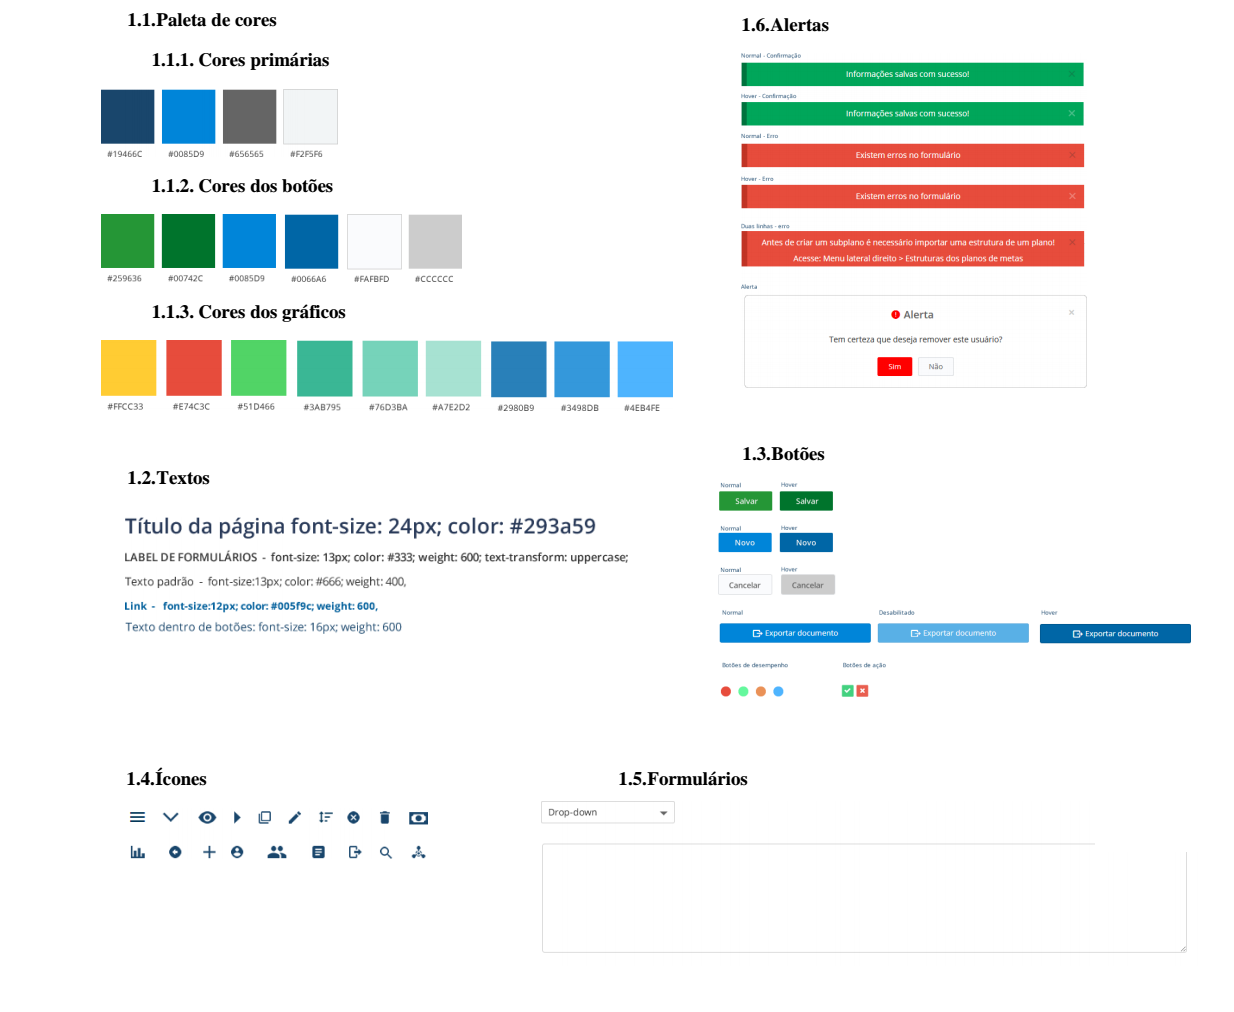
\includegraphics[width=1.1\textwidth]{images/estilo.png}
\caption{Estilo de design}
\label{fig:estilo}
\end{figure}


\section{Produto final}
\subsection{Usuários}
O software possui 4 visões de usuários diferentes, cada um com suas devidas permissões de acesso ao sistema. Para cada tipo de usuário foi pensado em um painel de bordo diferente, a fim de atender as informações relevantes àquele específico usuário. O painel de bordo representa as informações em forma visual, por meio de gráficos, tabelas e outros elementos, organizando os dados de uma forma simplificada e sob demanda às necessidades de cada usuário. Foram desenvolvidos diagramas de fluxo de trabalho, como demonstrado na Figura \ref{fig:workflow} para ajudar a entender o fluxo de navegação por parte de cada usuário.

% alterar essa figura
\begin{figure}[H]
\centering
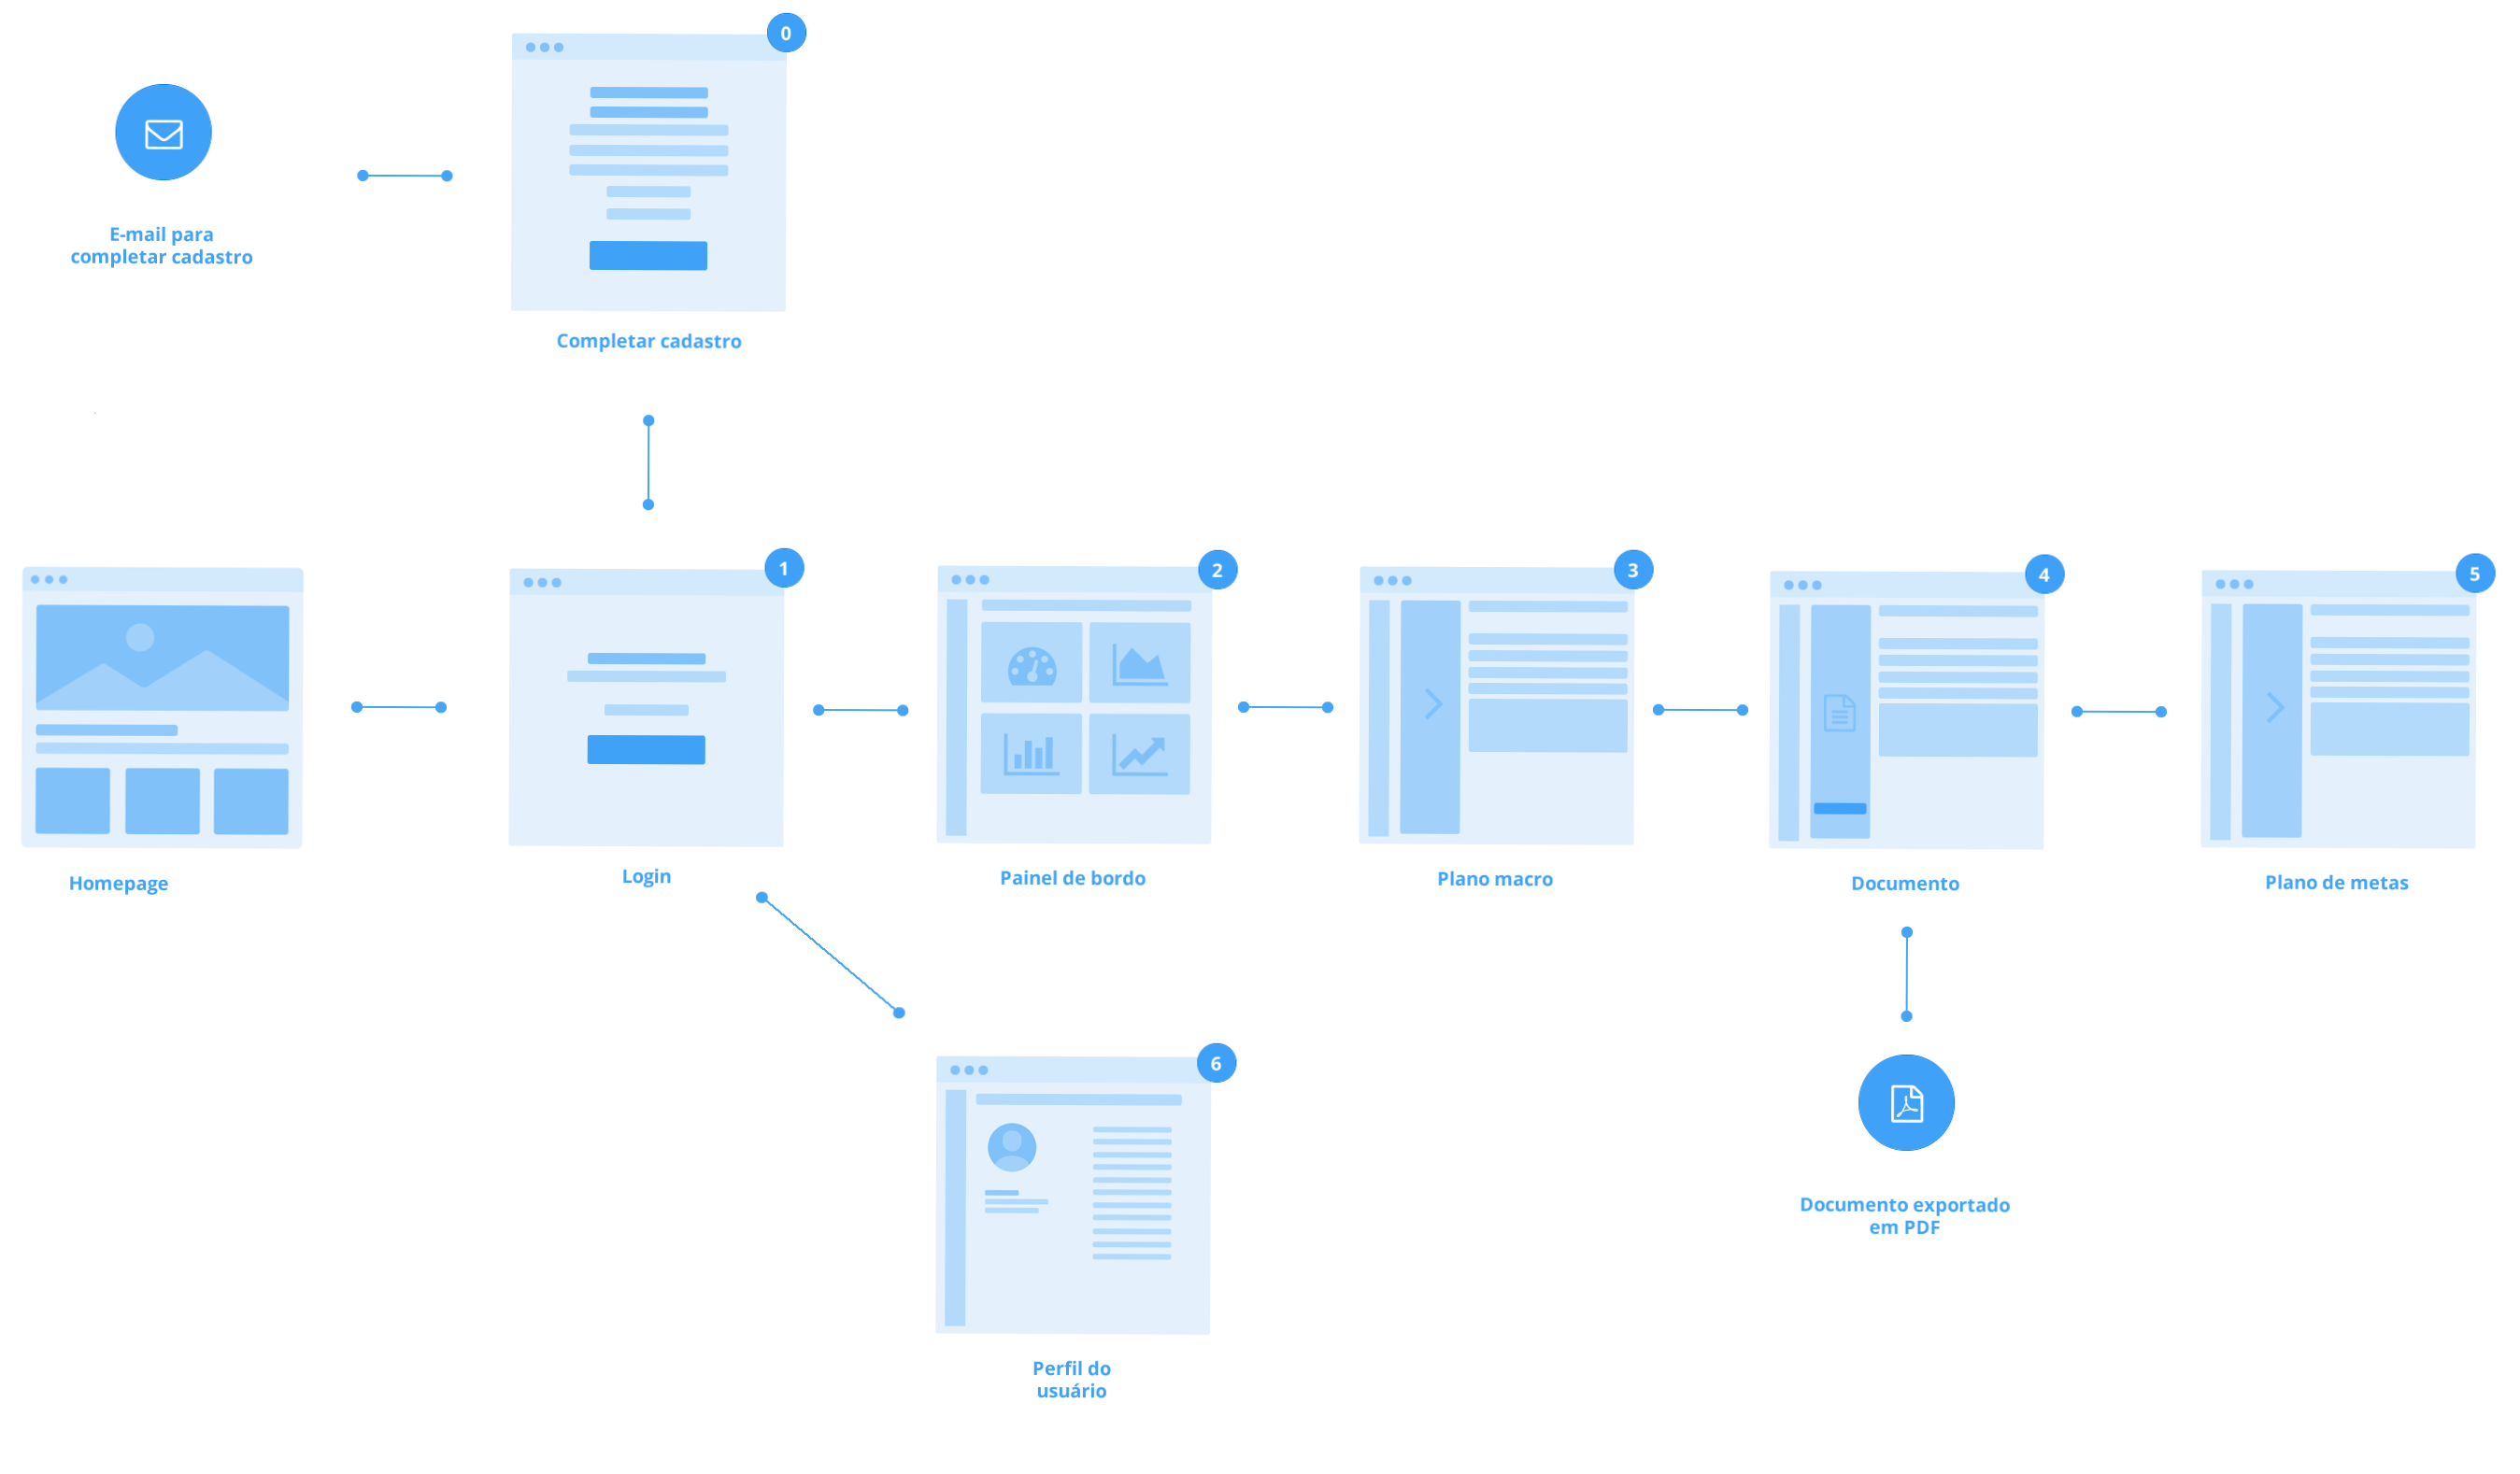
\includegraphics[width=1.1\textwidth]{images/flowwork.png}
\caption{Exemplo de diagrama de fluxo de trabalho}
\label{fig:workflow}
\end{figure}


\subsection{Estrutura dos dados}
A estrutura dos dados do planejamento estratégico é representada em níveis hierárquicos. A solução encontrada para a disposição dos dados foi em forma de árvore. Para facilitar o cadastro inicial, o usuário poderá cadastrar toda a estrutura diretamente na área da árvore do plano de metas do planejamento estratégico, com a possibilidade de editá-la no momento do cadastro ou em outro momento oportuno. 

O software possibilita importar uma estrutura do plano de metas, cada instituição ou empresa que utilizá-lo poderá torná-lo personalizado de acordo com suas estruturas de planejamento.

Após importar a estrutura, é possível cadastrar um plano macro, que contém todos os planos de metas da instituição. Cada plano de meta utiliza a estrutura importada para definir sua hierarquia. Juntamente com o plano de metas, é possível realizar a criação do documento do planejamento, e exportá-lo.


\subsection{Documento}
Ao criar um plano macro, o sistema cria uma estrutura pré-definida do documento do planejamento estratégico. A estrutura do documento é composta pelas seções e subseções seguindo o documento de referência proposto pelo cliente. A estrutura estará vazia, apenas com os títulos das seções e subseções, e os campos. O usuário poderá adicionar os campos personalizados de acordo com suas necessidades. Após o preenchimento do documento, o usuário poderá exportá-lo em formato PDF.












